\chapter{Propuesta de modificaciones al componente de AutoML para pre-procesado}\label{chap:2}
En el presente capítulo, se propone una serie de modificaciones destinadas a mejorar el componente AutoML Clasificación (pre-procesado). Estas modificaciones se centran en el pre-procesamiento de datos, incluyendo la automatización de tareas como la discretización, normalización y el tratamiento de valores únicos, valores de alta cardinalidad y valores faltantes. Además, se explorará la inclusión de técnicas de Optimización de Hiperparámetros (HPO) para encontrar configuraciones óptimas para los modelos. El enfoque principal de esta propuesta es la integración de estas dos facetas con el componente AutoML existente para clasificación. A lo largo de este capítulo, se describirá cómo estas modificaciones buscan mejorar la eficiencia y precisión del proceso de AutoML, creando modelos de clasificación más sólidos y adaptados a las necesidades específicas de los datos.

\section{Modificaciones en el pre-procesado}
Con el fin de abordar las problemáticas presentadas en el epígrafe \ref{epig:componente-ernesto}, se llevaron a cabo una serie de modificaciones sustanciales en el proceso de pre-procesamiento de datos. Estas adaptaciones se centraron en la automatización de la discretización y normalización, así como en el tratamiento de valores únicos, valores de alta cardinalidad y valores faltantes. En lo que respecta a la discretización y normalización, se implementaron técnicas automatizadas para garantizar una uniformidad en la escala y distribución de los datos, lo que contribuye a mejorar la precisión del modelado. Para abordar los valores únicos y de alta cardinalidad, se desarrollaron estrategias específicas que permitieron una gestión más efectiva de estas categorías, evitando la pérdida de información esencial y reduciendo el riesgo de sobreajuste. Por último, se implementaron métodos especializados para tratar los valores faltantes, asegurando que los datos incompletos no comprometieran la calidad del análisis. En las secciones siguientes, se detalla el funcionamiento y modelado de estas modificaciones con mayor profundidad.


\subsection{Discretización de variables numéricas} 
La discretización de variables numéricas se utiliza para convertir datos continuos en datos discretos, lo que permite que los algoritmos de aprendizaje automático puedan procesarlos y analizarlos adecuadamente. La discretización también puede mejorar la precisión de los modelos de aprendizaje automático al reducir el ruido en los datos y hacer que los patrones sean más fáciles de detectar. En aras de automatizar este proceso, se propone el subcomponente \textit{Discretizer} (Figura \ref{fig:subcomp-disc}).

\begin{figure}[H]
	\centering
	\includegraphics[width=0.15\linewidth]{"figuras/capi 2/subcomp-disc"}
	\caption[Subcomponente Discretizer]{Subcomponente \textit{Discretizer}}
	\label{fig:subcomp-disc}
\end{figure}

El subcomponente \textit{Discretizer} toma en su puerto de entrada los datos en formato tabular. Dichos datos, de tipo numéricos, son procesados por varios algoritmos de discretización y, como puerto de salida, se obtienen discretizados acorde al método de discretización con mejor precisión. Tiene una única restricción: no pueden tener valores perdidos como entrada. El diagrama de flujo de la figura \ref{fig:discretizacion} expone el flujo general del componente \textit{Discretizer}. El flujo KNIME correspondiente está presente en el anexo \ref{anex:flujo-disc-comp-id3}.

\begin{figure}[H]
	\centering
	\includegraphics[width=1\linewidth]{"figuras/capi 2/preprocesado/discretizacion.drawio"}
	\caption{Diagrama de flujo general de Discretizer}
	\label{fig:discretizacion}
\end{figure}

Para la discretización se emplean los nodos presentes en la figura \ref{fig:discretizacion-nodos}. El nodo \textit{Auto-Binner} contiene tres métodos de discretización: \textit{Equal-Width, Equal-Frequency} y \textit{Quantile-Based}; mientras el nodo \textit{CAIM Binner} contiene el método \textit{CAIM}. Para la elección de los \textit{k} intervalos se emplea la Regla de Sturges, descrita en la sección \ref{sub-epigrafe-disc}. El nodo \textit{CAIM Binner} no requiere una configuración en específico, y para el método Quantile-Based se escogieron los cuantiles por defecto, es decir 0.0, 0.25, 0.5, 0.75 y 1.0.

\begin{figure}[H]
	\centering
	\begin{subfigure}[b]{0.25\linewidth}
		\centering
		\includegraphics[width=0.5\linewidth]{"figuras/capi 2/auto-binner-nodo"}
		\caption{Nodo \textit{Auto-Binner}}
		\label{fig:auto-binner-nodo}
	\end{subfigure}
	\hspace{1.5cm}
	\begin{subfigure}[b]{0.25\linewidth}
		\centering
		\includegraphics[width=0.5\linewidth]{"figuras/capi 2/caim-binner-nodo"}
		\caption{Nodo \textit{CAIM Binner}}
		\label{fig:caim-binner-nodo}
	\end{subfigure}
	\caption{Nodos empleados para la discretización}
	\label{fig:discretizacion-nodos}
\end{figure}

Tras discretizar el conjunto de datos con cada método correspondiente, se aplica el modelo en cuestión a cada uno de los datos resultantes, con el objetivo de compararlos en cuanto a precisión y Cohen's Kappa, y escoger el algoritmo con mejor desempeño. 

\subsection{Pre-procesado de variables de tipo \textit{string}}
Los valores nominales únicos, o categorías con un solo ejemplo en una columna, pueden parecer insignificantes a primera vista, pero su correcto manejo es esencial para evitar posibles problemas de calidad de datos y garantizar la integridad de los análisis. El Componente AutoML Clasificación (pre-procesado) poseía un tratamiento erróneo de estos valores, al eliminar las columnas nominales que superaban un umbral determinado de categorías distintas. \\ 
En aras de depurar estas inconsistencias, el diagrama de la figura \ref{fig:string-preprocs} muestra un nuevo flujo para el pre-procesado de String, donde la actividad de color amarillo expresa que se modificó la que anteriormente se encontraba en el componente; mientras que la actividad en verde refleja una nueva implementación.

\begin{figure}[H]
	\centering
	\includegraphics[width=0.95\linewidth]{"figuras/capi 2/preprocesado/string preprocs.drawio"}
	\caption{Diagrama de flujo para el pre-procesado de string}
	\label{fig:string-preprocs}
\end{figure}

A continuación se exponen los cambios realizados al componente String preprocs:
\begin{itemize}
	\item Eliminar valores únicos por columna:  Se enmienda el error antes expuesto, al modificar el subcomponente "filtrar valores únicos", implementando la eliminación de las columnas donde más del 80\% de los valores son únicos.
	\item Reemplazar con otros: En este nuevo componente, los valores únicos en una columna que representan una minoría, son reemplazados por la categoría 'otros'.  Para ello, iterando por cada columna dentro de un ciclo, se calculan la frecuencia absoluta y relativa de cada atributo, y aquellos que representen menos del 1\% son los elegidos para la sustitución por la nueva categoría. 
\end{itemize}
El flujo KNIME de los nuevos subcomponentes se encuentran en los ANEXOS X y Y.


\subsection{Manejo de valores faltantes}
El tratamiento de valores faltantes en conjuntos de datos es un paso crítico en la preparación y análisis de datos. La presencia de datos faltantes puede afectar significativamente la calidad y la fiabilidad de cualquier análisis o modelo que se derive de ellos. Adicionalmente, algunos algoritmos requieren que no existan valores faltantes para su funcionamiento. En aras de mejorar la imputación de estos valores, se propone modificar el subcomponente 'Valores faltantes', cuyo diagrama de flujo se presenta en la figura \ref{fig:valores-faltantes}.

\begin{figure}[H]
	\centering
	\includegraphics[width=1\linewidth]{"figuras/capi 2/preprocesado/valores faltantes.drawio"}
	\caption{Diagrama de flujo para el manejo de valores faltantes}
	\label{fig:valores-faltantes}
\end{figure}

La imputación de valores faltantes ha sido modificada, por los motivos expuestos en la sección \ref{secc:mv}. En la figura \ref{fig:mv-imputation} se presenta el diagrama de flujo de la nueva implementación para la sustitución de estos valores. 

\begin{figure}[H]
	\centering
	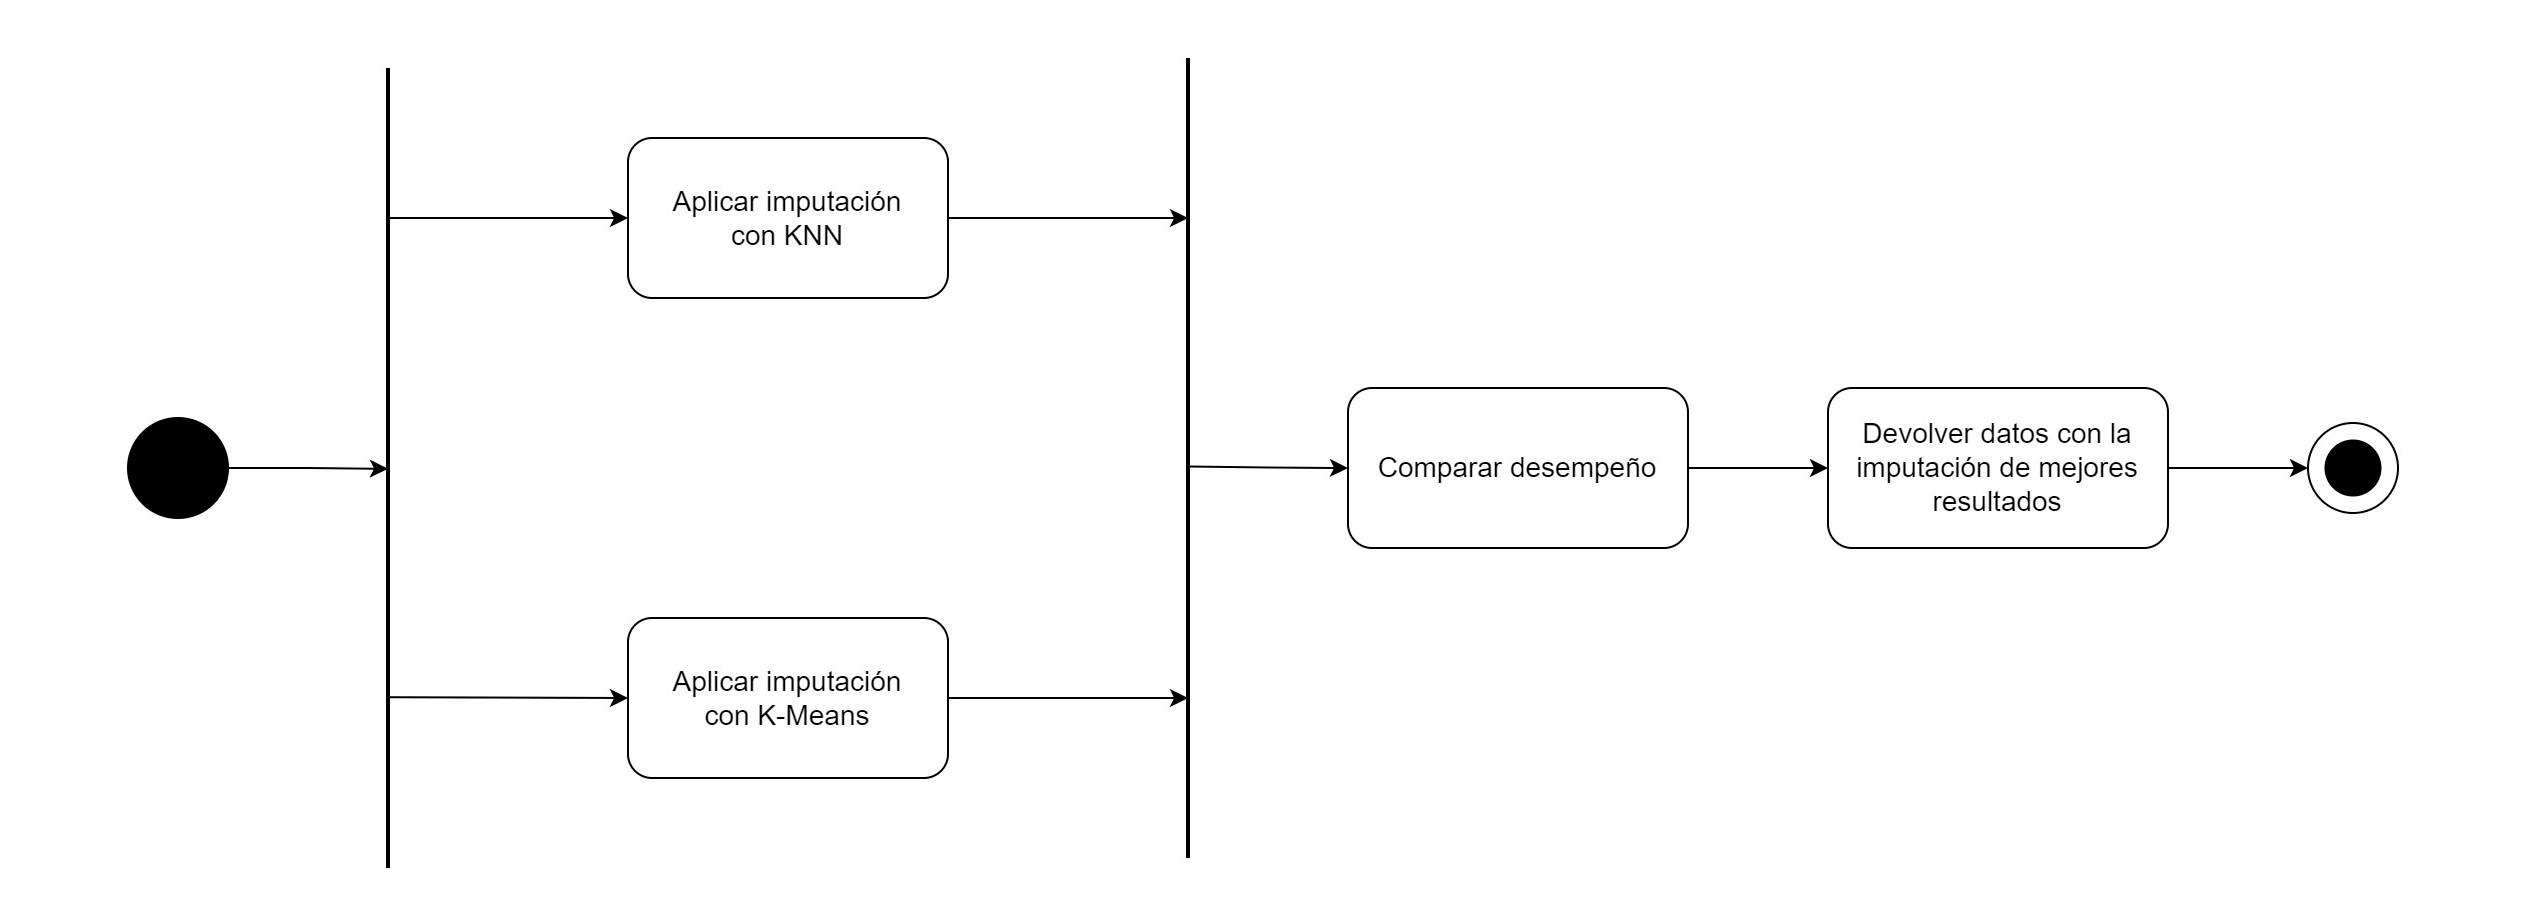
\includegraphics[width=1\linewidth]{"figuras/capi 2/preprocesado/mv imputation.drawio"}
	\caption{Diagrama de flujo para la imputación de valores faltantes}
	\label{fig:mv-imputation}
\end{figure}

Primeramente se aplican en paralelo las técnicas de imputación KNN y K-Means, al terminar se aplica el algoritmo de aprendizaje automático en cuestión con los datos imputados por cada método y, finalmente, se comparan los resultados acorde a las métricas Precisión y Cohen's Kappa, para devolver los datos con la mejor sustitución. En el ANEXO X se muestra el flujo KNIME de estas estrategias. 

\subsection{Codificación y normalización}
La codificación de variables categóricas implica asignar valores numéricos a estas categorías para que los algoritmos de aprendizaje automático puedan trabajar con ellas. Este es el propósito del subcomponente "Pre-procesar números", además de la normalización de variables numéricas. En aras de clarificar el funcionamiento de este proceso, se decide renombrarlo a "Codificar y normalizar".\\
La normalización son proporciones sin unidades de medida (adimensionales o invariantes de escala) que nos permiten poder comparar elementos de distintas variables y distintas unidades de medida. Esta es necesaria para cambiar los valores de las columnas numéricas del conjunto de datos para usar una escala común, sin distorsionar las diferencias en los intervalos de valores ni perder información. La normalización es fundamental para que algunos algoritmos modelen los datos correctamente. \\
En KNIME es posible implementar la normalización a partir del nodo "Normalizer". En este nodo se encuentran tres métodos para normalizar, a elección del usuario: Decimal Scaling, Z-Score y Min-Max. Este proceso se encuentra en el subcomponente para el pre-procesado de números, cuyo diagrama de flujo se presenta en la figura \ref{fig:number-preprocs}.
Por otro lado, los valores de alta cardinalidad, aquellos que se repiten con frecuencia y pueden ser numerosos, son cruciales para comprender tendencias y patrones en los datos. La codificación de estas variables se refiere a técnicas especiales de codificación que se utilizan cuando tienes variables categóricas con un gran número de categorías o niveles distintos. La alta cardinalidad puede dificultar la gestión de estas variables en modelos de aprendizaje automático, y es importante abordarlas de manera eficiente. \\

\begin{figure}[H]
	\centering
	\includegraphics[width=1\linewidth]{"figuras/capi 2/preprocesado/number preprocs.drawio"}
	\caption{Diagrama de flujo del pre-procesado para la codificación y normalización}
	\label{fig:number-preprocs}
\end{figure}

A continuación se exponen los cambios realizados al pre-procesado para la codificación y normalización:

\begin{itemize}
	\item Codificar con One-Hot Encoding: Para el tratamiento de valores con alta cardinalidad, se emplea la codificación One-Hot, utilizando el nodo One To Many. Para esto se escogen los atributos que tienen como mínimo 15 categorías distintas. Dado que esta técnica produce gran dimensionalidad, se utilizan para su reducción los métodos
	\begin{enumerate}
		\item filtrar por varianza, utilizando el nodo Low Variance Filter, donde las columnas creadas con una varianza menor a 0.01 son eliminadas; y 
		\item filtrar por correlación, utilizando el nodo Correlation Filter, donde las columnas con una correlación mayor a 0.9 son eliminadas.
	\end{enumerate}
	\item Normalizar: En aras de automatizar este proceso, se propone el subcomponente "Normalizer", de igual nombre al nodo nativo de KNIME, en donde se encuentra el nodo Normalizer de la herramienta para la comparación de los métodos que contiene, en función de un modelo predeterminado. En la figura \ref{fig:normalizacion} se presenta el diagrama de flujo de este subcomponente. 
\end{itemize}


\begin{figure}[H]
	\centering
	\includegraphics[width=1\linewidth]{"figuras/capi 2/preprocesado/normalizacion.drawio"}
	\caption{Diagrama de flujo para la normalización}
	\label{fig:normalizacion}
\end{figure}

Siguiendo el mismo esquema del subcomponente "Discretizer", tras aplicar la normalización con los distintos métodos ofrecidos por la herramienta KNIME, se aplica el algoritmo de aprendizaje automático que requiere los datos normalizados y, posteriormente, se realiza la evaluación del desempeño de cada uno, acorde a la precisión y el Cohen's Kappa. Luego de escoger el mejor, se devuelve la tabla con los datos normalizados.



\section{Componente AutoML Clasificación (Optimización de hiperparámetros)}
Antes de explorar en detalle las adaptaciones realizadas en cada modelo, es fundamental presentar el Componente AutoML Clasificación (Optimización de hiperparámetros), con el objetivo de facilitar el entendimiento en los epígrafes posteriores. 

\textbf{tooooodo lo que lleva con sus epígrafes, esto es lo que estaba en las practicas}

El componente propuesto, presente en la figura \ref{fig:automl-componente-hpo}, para la optimización de hiperparámetros, contiene la siguiente configuración:
\begin{figure}[H]
	\centering
	\includegraphics[width=0.35\linewidth]{"figuras/capi 2/automl-componente-hpo"}
	\caption[Componente AutoML Clasificación (Optimización de Hiperparámetros)]{Componente \textit{AutoML Clasificación (Optimización de Hiperparámetros)}}
	\label{fig:automl-componente-hpo}
\end{figure}
\begin{enumerate}
	\item Puerto de entrada: recibe los datos de entrada en formato tabular.
	\item Elementos de la configuración:
	\begin{itemize}
		\item Columna objetivo: presenta las columnas de tipo \textit{string} que pueden fungir como columna objetivo.
		\item Estrategia de optimización de hiperparámetros: se selecciona la estrategia de optimización de hiperparámetros entre las disponibles (Random Search, Bayesian Optimization (TPE), Brute Force y Hillclimbing).
		\item Selección del número de subconjuntos de la validación cruzada: el valor introducido determina la cantidad de veces que se divide el conjunto de datos en subconjuntos de entrenamiento y prueba, durante el proceso de validación.
	\end{itemize}
	\item Puerto de salida: tabla de hiperparámetros optimizados, siguiendo la estrategia de optimización escogida.
\end{enumerate}

\subsection{Uso y configuración del componente AutoML Clasificación (Optimización de Hiperparámetros)}
A continuación, se define la secuencia de pasos para el correcto funcionamiento del componente \textit{AutoML Clasificación (Optimización de Hiperparámetros)}:

\begin{enumerate}
	\item Proporcionar el conjunto de datos al puerto de entrada (el componente marcará error en este punto, pues la configuración es obligatoria).
	\item Dar click derecho sobre el componente, seleccionar “Configure…”. 
	\item Seleccionar la configuración deseada (como se observa en el ejemplo de la figura \ref{fig:config-automl-hpo}). 
	\item Ejecutar el componente (inicialmente el puerto de salida se encuentra vacío).
	\item Dar click derecho sobre el componente y seleccionar “Interactive View: AutoML” (Fig3). 
\end{enumerate}

\begin{figure}[H]
	\centering
	\includegraphics[width=0.5\linewidth]{"figuras/capi 2/config-automl-hpo"}
	\caption[Ejemplo de configuración del componente AutoML (Optimización de Hiperparámetros)]{Ejemplo de configuración del componente \textit{AutoML (Optimización de Hiperparámetros)}}
	\label{fig:config-automl-hpo}
\end{figure}

\begin{figure}[H]
	\centering
	\includegraphics[width=0.5\linewidth]{"figuras/capi 2/automl-hpo-vista-salida"}
	\caption[Vista de la salida.]{Vista de la salida.}
	\label{fig:automl-hpo-vista-salida}
\end{figure}

\subsection{Requisitos y restricciones del componente AutoML Clasificación (Optimización de Hiperparámetros)}
El componente propuesto debe cumplir los siguientes requisitos funcionales:

\begin{itemize}
	\item RF1: El componente debe permitir seleccionar columna objetivo
	\item RF2: El componente debe permitir seleccionar estrategia de optimización de hiperparámetros.
	\item RF3: El componente debe permitir seleccionar cantidad de subconjuntos en la validación cruzada.
	\item RF4: El componente debe optimizar hiperparámetros y entrenar datos para Redes Neuronales de Retro propagación.
	\item RF5: El componente debe retornar tabla de hiperparámetros optimizados.
\end{itemize}

El componente propuesto presenta las siguientes restricciones para su funcionamiento:

\begin{itemize}
	\item Los datos de entrada deben encontrarse en formato tabular.
	\item La columna objetivo debe ser de tipo \textit{string}.
	\item Los datos de entrada deben ser de tipo numérico, a excepción de la columna objetivo.
	\item Los datos numéricos deben estar previamente normalizados.
\end{itemize}

\subsection{Modelación del componente AutoML Clasificación (Optimización de Hiperparámetros)}
El diagrama de flujo de la figura \ref{fig:diagrama-flujo-gral-comp-hpo} expone el flujo general del componente \textit{AutoML Clasificación (Optimización de Hiperparámetros)}.

\begin{figure}[H]
	\centering
	\includegraphics[width=0.7\linewidth]{"figuras/capi 2/diagrama-flujo-gral-comp-hpo"}
	\caption[Diagrama de flujo general del componente AutoML Clasificación (Optimización de Hiperparámetros)]{Diagrama de flujo general del componente \textit{AutoML Clasificación (Optimización de Hiperparámetros)}}
	\label{fig:diagrama-flujo-gral-comp-hpo}
\end{figure}

La configuración de la selección de parámetros es el primer paso, en el cual se crearán las variables que dictarán el comportamiento del flujo. Posteriormente, se ejecuta la optimización de hiperparámetros para RProp, donde recoge los resultados en una tabla y luego los grafica. El flujo KNIME correspondiente se evidencia en el Anexo \ref{aped.flujo-hpo-rprop}.

\subsubsection{Selección de parámetros}
Los parámetros que rigen el funcionamiento del componente propuesto, brindan al usuario una mayor personalización de la optimización de hiperparámetros, pues le ofrece la libertad de configurar múltiples factores claves de esta etapa. El diagrama de actividades de la figura \ref{fig:diagrama-act-selecc-param-hpo} expone el flujo para la selección de parámetros.

\begin{figure}[H]
	\centering
	\includegraphics[width=0.7\linewidth]{"figuras/capi 2/diagrama-act-selecc-param-hpo"}
	\caption[Diagrama de actividades de selección de parámetros]{Diagrama de actividades de selección de parámetros}
	\label{fig:diagrama-act-selecc-param-hpo}
\end{figure}

La selección de parámetros se realiza con los siguientes nodos de configuración, presentes en el repositorio base:

\begin{itemize}
	\item Seleccionar columna objetivo: se emplea el nodo \textit{Column Selection Configuration}, el cual recibe una tabla y devuelve el nombre de la columna seleccionada como variable de flujo. En este caso, presenta la configuración adicional para solo mostrar las columnas de tipo \textit{string}.
	\item Seleccionar estrategia de optimización de hiperparámetros: la selección de la estrategia se lleva a cabo empleando el nodo \textit{Single Selection Configuration}. Devuelve la variable \texttt{strategy} con el valor seleccionado previamente.
	\item Seleccionar número de subconjuntos en la validación cruzada: la selección de la cantidad de subconjuntos de partición de entrenamiento, se lleva a cabo con el nodo \textit{Integer Configuration}. Este devuelve la variable de flujo resultante de la selección, en este caso presenta la configuración para limitar el rango entre 5 y 10.
\end{itemize}

\subsection{Optimización de hiperparámetros para RProp}
Las Redes Neuronales por Retro-propagación necesitan que todos los valores sean de tipo numéricos y estos se encuentren normalizados. Para el entrenamiento y prueba de las Redes Neuronales por Retro-propagación, se emplean los nodos \textit{RProp MLP Learner} y \textit{MultiLayerPerceptron Predictor} respectivamente.
El diagrama de actividades de la figura \ref{fig:diagrama-act-proc-rprop-hpo}, expone el flujo para el procesamiento necesario para la ejecución del algoritmo Redes Neuronales por Retropropagación, con optimización de hiperparámetros.
\begin{figure}[H]
	\centering
	\includegraphics[width=0.7\linewidth]{"figuras/capi 2/diagrama-act-proc-rprop-hpo"}
	\caption{Diagrama de actividades para el procesamiento de RProp con HPO}
	\label{fig:diagrama-act-proc-rprop-hpo}
\end{figure}

Para llevar a cabo el procesamiento RProp se emplean los siguientes nodos: 
\begin{itemize}
	\item Ciclo para recorrer el rango de hiperparámetros: se emplean los nodos \textit{Parameter Optimization Loop Start} y \textit{Parameter Optimization Loop End} (Figura \ref{fig:nodos-param-opt-loop}). Ambos permiten guardar todas las iteraciones realizadas por el algoritmo con las diferentes combinaciones de hiperparámetros. Para su configuración, se eligieron como hiperparámetros el número de capas, la cantidad de neuronas y el número máximo de iteraciones (Figura \ref{fig:conf-nodo-param-loop}).
	\begin{figure}[H]
		\centering
		\includegraphics[width=0.5\linewidth]{"figuras/capi 2/nodos-param-opt-loop"}
		\caption[Nodos Parameter Optimization Loop Start y Parameter Optimization Loop End]{Nodos \textit{Parameter Optimization Loop Start} y \textit{Parameter Optimization Loop End}}
		\label{fig:nodos-param-opt-loop}
	\end{figure}
	
	\begin{figure}[H]
		\centering
		\includegraphics[width=0.6\linewidth]{"figuras/capi 2/conf-nodo-param-loop"}
		\caption[Configuración del nodo Parameter Optimization Loop Start]{Configuración del nodo \textit{Parameter Optimization Loop Start}}
		\label{fig:conf-nodo-param-loop}
	\end{figure}
	
	\item Ciclo para dividir el conjunto de datos: se emplean los nodos \textit{X-Partitioner} y \textit{X-Aggregator}, para dividir el conjunto de datos en \textit{k} particiones y realizar una validación cruzada, donde cada partición se utiliza como conjunto de prueba una vez y las otras \textit{k-1} particiones se utilizan como conjunto de entrenamiento.
	\item Calcular la exactitud: se emplea el nodo \textit{Scorer}, el cual recibe la predicción y la columna objetivo en una tabla para la evaluación. 
	\item Graficar: se emplea el nodo \textit{Table View}, capaz de visualizar la tabla de los hiperparámetros con mejor resultado.	
\end{itemize}


\subsection{Optimización de hiperparámetros para PNN}
blablabla
blablabla

\subsection{Optimización de hiperparámetros para SVM}

blablabla

\subsection{Optimización de hiperparámetros para Random Forest}
blablabla



\section{Modelación de nueva versión del componente AutoML Clasificación}
El enfoque principal de esta propuesta es la integración de los subcomponentes desarrollados para el pre-procesado y el componente AutoML Clasificación (Optimización de hiperparámetros) con el componente AutoML existente para clasificación, cuyo diagrama de flujo se presenta en la FIGURA X DIAGRAMA ERNESTO. \\

\textbf{FOTO DEL DIAGRAMA DE FLUJO DEL COMPONENTE} \\

Como se puede apreciar en el diagrama de flujo de la FIGURA X DIAGRAMA ERNESTO, se implementa un nuevo modelo para la clasificación: Random Forest. Ademas, se realizan cambios en la personalización del componente: la eliminación del umbral de valores únicos por columna y un nuevo campo para la elección de la estrategia de optimización que se utilizará para la optimización de hiperparámetros. Estos cambios se pueden observar en la FIGURA X PERSONALIZACION DEL COMPONENTE. \\

\textbf{ FIGURA X PERSONALIZACION DEL COMPONENTE} \\

Con el propósito de abordar la integración con las nuevas implementaciones, se discutirán detalladamente en las secciones siguientes.

\subsection{Procesado de ID3}
El algoritmo ID3 se puede ejecutar en KNIME a través del nodo Id3 (3.7), el cual forma parte de una extensión de la herramienta Weka. Al no ser un nodo nativo en KNIME, no es posible optimizar los hiperparámetros del mismo, sin embargo se realizaron las integraciones con los componentes de pre-procesado discutidos en las secciones posteriores. Esto se manifiesta en el diagrama de flujo presente en la figura \ref{fig:procesado-id3}.

\begin{figure}[H]
	\centering
	\includegraphics[width=1\linewidth]{"figuras/capi 2/modelos/procesado id3.drawio"}
	\caption{Diagrama de flujo del procesamiento del modelo ID3}
	\label{fig:procesado-id3}
\end{figure}

Tal como se puede apreciar en la figura \ref{fig:procesado-id3}, simplemente se realizaron las modificaciones pertinentes en el manejo de valores faltantes, la discretización y el pre-procesado de String.

\subsection{Procesado para C4.5}
El algoritmo C4.5, al igual que Id3, forma parte de la extensión Weka y no permite la incorporación de la optimización de hiperparámetros. Las modificaciones efectuadas en el pre-procesado están presentes en el diagrama de flujo de la figura \ref{fig:procesado-c4pt5}.

\begin{figure}[H]
	\centering
	\includegraphics[width=1\linewidth]{"figuras/capi 2/modelos/procesado c4pt5.drawio"}
	\caption{Diagrama de flujo del procesamiento del modelo C4.5}
	\label{fig:procesado-c4pt5}
\end{figure}

Como se observa, estas modificaciones fueron las mismas que a su predecesor, con la diferencia de que, en la versión anterior del componente AutoML Clasificación (pre-procesado), en este modelo no estaba presente la discretización, ya que es versátil y puede manejar tanto variables categóricas como variables numéricas. Sin embargo, se decide incorporarla ya que, a pesar de lo anteriormente dicho, C4.5 puede ser menos eficaz cuando se utiliza en conjuntos de datos con datos numéricos muy dispersos. En tales casos, los árboles de decisión pueden requerir una mayor profundidad para capturar patrones en las variables numéricas, lo que puede llevar a árboles más complejos y propensos al sobreajuste. 

\subsection{Procesado para CART}
El algoritmo CART tiene los mismos requisitos que C4.5 para su ejecución, por lo que la diferencia entre ambos es el nodo que ejecuta el algoritmo, pues emplea el nodo SimpleCart (3.7). La unica diferencia es que no se emplea la discretizacion de variables numericas, ya que este arbol de decision puede ser empleado tanto en tareas de clasificacion como de regresion, lo que causa que funcione de manera efectiva tanto con datos numericos como nominales. Por otra parte, al formar parte de la extensión Weka, este nodo tampoco presenta la optimización de hiperparámetros. \\
En la figura \ref{fig:procesado-cart} se presenta el diagrama de flujo del procesado del algoritmo CART.

\begin{figure}[H]
	\centering
	\includegraphics[width=1\linewidth]{"figuras/capi 2/modelos/procesado cart.drawio"}
	\caption{Diagrama de flujo del procesado de CART}
	\label{fig:procesado-cart}
\end{figure}


\subsection{Procesamiento para Random Forest}
Dado que los modelos de arboles de decisión empleados en el componente AutoML Clasificación (pre-procesado) forman parte de extensiones Weka y, por tal motivo, no se puede ejecutar la optimización de hiperparámetros, se decide agregar un nuevo modelo: Random Forest. Este algoritmo puede trabajar con una amplia variedad de tipos de datos, ya sean datos numéricos o categóricos. Esto hace que Random Forest sea una elección versátil para tareas de clasificación y regresión. Por ello, el pre-procesado de este algoritmo es igual al de CART. \\
El diagrama de flujo del procesado de este nuevo modelo se muestra en la figura \ref{fig:procesado-rf}.

\begin{figure}[H]
	\centering
	\includegraphics[width=1\linewidth]{"figuras/capi 2/modelos/procesado rf.drawio"}
	\caption{Diagrama de flujo del procesamiento de Random Forest}
	\label{fig:procesado-rf}
\end{figure}


\subsection{Procesamiento para Redes Neuronales por Retropropagación}
Las Redes Neuronales por Retropropagación necesitan procesar los valores numéricos, además de los procesamientos realizados para C4.5 y CART, dado que solo permiten atributos numéricos. Por esta razón, se incluye el subcomponente para la codificación y normalización, tal como se muestra en el diagrama de flujo de la figura \ref{fig:procesado-rprop}. Por otra parte, también se implementa la optimizacion de hiperparametros al integrar el componente AutoML Clasificación (Optimización de hiperparámetros).

 \begin{figure}[H]
	\centering
	\includegraphics[width=1\linewidth]{"figuras/capi 2/modelos/procesado rprop.drawio"}
	\caption{Diagrama de flujo del procesamiento de RProp}
	\label{fig:procesado-rprop}
\end{figure}



\subsection{Procesamiento para Redes Neuronales Probabilísticas}
Las Redes Neuronales Probabilísticas, al igual que RProp, trabajan con atributos numéricos. Por ello, se decide incorporar la codificación y normalización, la cual estaba en la versión anterior, sin embargo la normalización no se encontraba. Como en RProp, se implementa la optimización de hiperparámetros al integrar el componente AutoML Clasificación (Optimización de hiperparámetros). En la figura \ref{fig:procesado-pnn} se muestra el diagrama de flujo de procesamiento de PNN.

\begin{figure}[H]
	\centering
	\includegraphics[width=1\linewidth]{"figuras/capi 2/modelos/procesado pnn.drawio"}
	\caption{Diagrama de flujo para el procesado de PNN}
	\label{fig:procesado-pnn}
\end{figure}


\subsection{Procesamiento para SVM}
En este algoritmo, al igual que en las redes neuronales, se trabaja con atributos numéricos. No obstante, como fue el caso de PNN, no se encontraba la normalización de variables numéricas, que a pesar de no ser un requisito por el algoritmo, es un paso clave para su desempeño. Por otra parte, se implementa la optimización de hiperparámetros al integrar el componente AutoML Clasificación (Optimización de hiperparámetros). El diagrama de flujo para el procesamiento de SVM se muestra en la figura \ref{fig:procesado-svm}.

\begin{figure}[H]
	\centering
	\includegraphics[width=1\linewidth]{"figuras/capi 2/modelos/procesado svm.drawio"}
	\caption{Diagrama de flujo del procesamiento de SVM}
	\label{fig:procesado-svm}
\end{figure}




\section{Conclusiones parciales}
A partir de lo analizado en este capítulo, se arriba a las siguientes conclusiones:
\begin{itemize}
	\item Se obtiene el diseño de un subcomponente para la discretización de variables numéricas.
	\item Para la discretización, se implementan los métodos Equal-Width, Equal-Frequency, Quantile-Based y CAIM.
	\item La implementación de los métodos de discretización se realiza con los nodos nativos de KNIME \textit{Auto-Binner} y \textit{CAIM Binner}.
	\item Se obtiene el diseño del componente AutoML Clasificación (Optimización de hiperparámetros).
	\item Se describe el uso y  los diferentes requisitos y restricciones del componente AutoML Clasificación (Optimización de hiperparámetros).
	\item Se define el rango de hiperparámetros (Iteraciones, capas y número de neuronas) del algoritmo Rprop.
\end{itemize}

\pagebreak

